
\section{Organisation}

\begin{frame}
  {Roland Schäfer}
  \onslide<+->
  \begin{itemize}[<+->]
    \item seit WS 2022\slash 2023 Professur für Grammatik und Lexikon
    \item 2020--2022 Forschungsstelle an der HU Berlin
    \item 2018 habilitiert an der HU Berlin\\
      (Germanistische Linguistik und allgemeine Sprachwissenschaft)
    \item 2007--2022 Mitarbeiter an der FU Berlin
    \item 2008 promoviert an der Uni Göttingen (Englische Syntax)
    \item 2002--2007 Mitarbeiter in der Sprachwissenschaft in Göttingen
    \item Studium in Marburg (Sprachwissenschaft, Japanologie)
  \end{itemize}
  \Zeile
  \onslide<+->
  Bitte nennen Sie mich nicht Professor\ldots\ \onslide<+-> Wenn Sie es tun, dann bitte richtig:\\
  \url{https://rolandschaefer.net/regeln-fur-den-mailverkehr/}
\end{frame}

\begin{frame}
  {Forschung}
  \onslide<+->
  Linguistik (des Deutschen)\\
  \Halbzeile
  \onslide<+->
  \begin{itemize}[<+->]
    \item kognitiv fundierte Grammatik
    \item Morphosyntax und Graphematik
    \item grammatische Variation ("`Zweifelsfälle"')
    \item individuelle Variation
    \item Registervariation
    \item Epistemologie
  \end{itemize}
  \Zeile
  \onslide<+->
  Methoden\\
  \Halbzeile
  \onslide<+->
  \begin{itemize}[<+->]
    \item Korpuserstellung und -analyse
    \item verhaltensbasierte Experimente
    \item Fragen der statistischen Inferenz
  \end{itemize}
\end{frame}

\begin{frame}
  {Sitzungsverlauf}
  \onslide<+->
  \begin{itemize}[<+->]
    \item vorbereitende Lektüre: \citet{Schaefer2018b}
    \item 10--20 Minuten Besprechung der Take-Home-Übungen
    \item 20--30 Minuten interaktiver Vortrag
    \item 40--60 Minuten 
  \end{itemize}
\end{frame}

\section{Das Lexikon}

\begin{frame}
  {Lexika}
  \onslide<+->
  Was ist für Sie ein "`Lexikon"'?\\
  \Zeile
  \onslide<+->
  \onslide<+->
  \begin{itemize}[<+->]
    \item Buch
    \item \alert{Datenbank} + Datenstruktur
    \item Ort der Kodierung \alert{egal}
  \end{itemize}
\end{frame}

\begin{frame}
  {Inhalt\slash Daten in Lexika}
  \onslide<+->
  Was gehört für Sie in ein Lexikon? Und warum?\\
  \Zeile
  \onslide<+->
  \onslide<+->
  \begin{itemize}[<+->]
    \item phonetische\slash phonologische Information (über Wörter \ldots)\\
      \Viertelzeile
      \textit{Klee} \alert{[kleː]}
    \item morphologische Information\\
      \Viertelzeile
      \textit{Klee} [kleː] \alert{N mask.\ st.}
    \item (morpho-)syntaktische Information\\
      \Viertelzeile
      \textit{rennen} [ʁɛnən] V st.\ (\textit{rannte, gerannt}) \alert{itr.}
      \Halbzeile
    \item beim mentalen Lexikon ähnlich
      \Halbzeile
    \item \alert{Bedeutung?} \ldots nicht unbedingt \citep{Elman2009}
    \item Evidenz für einfache Verknüpfungen zwischen \alert{Formlexikon} und \alert{Weltwissen}
  \end{itemize}
\end{frame}

\section{Struktur im Lexikon | Bedeutung?}

\begin{frame}
  {Was heißt hier Struktur?}
  \onslide<+->
  Welche \alert{lexikalisch-semantischen Beziehungen} gibt es zwischen Wörtern?\\
  \onslide<+->
  \Halbzeile
  \begin{itemize}[<+->]
    \item Substantiv $\Leftrightarrow$ Substantiv
    \item Verb $\Leftrightarrow$ Verb
    \item Adjektiv $\Leftrightarrow$ Adjektiv
    \item Substantiv $\Leftrightarrow$ Verb
    \item \ldots
  \end{itemize}
  \onslide<+->
  \Zeile
  Ach, übrigens, merken Sie was? \onslide<+-> \alert{Substantiv, Verb, Adjektiv, \ldots}
\end{frame}

\begin{frame}
  {Lexikalische Semantik und Ontologie}
  \onslide<+->
  Was ist eine Ontologie?\\
  \onslide<+->
  \Zeile
  \centering 
  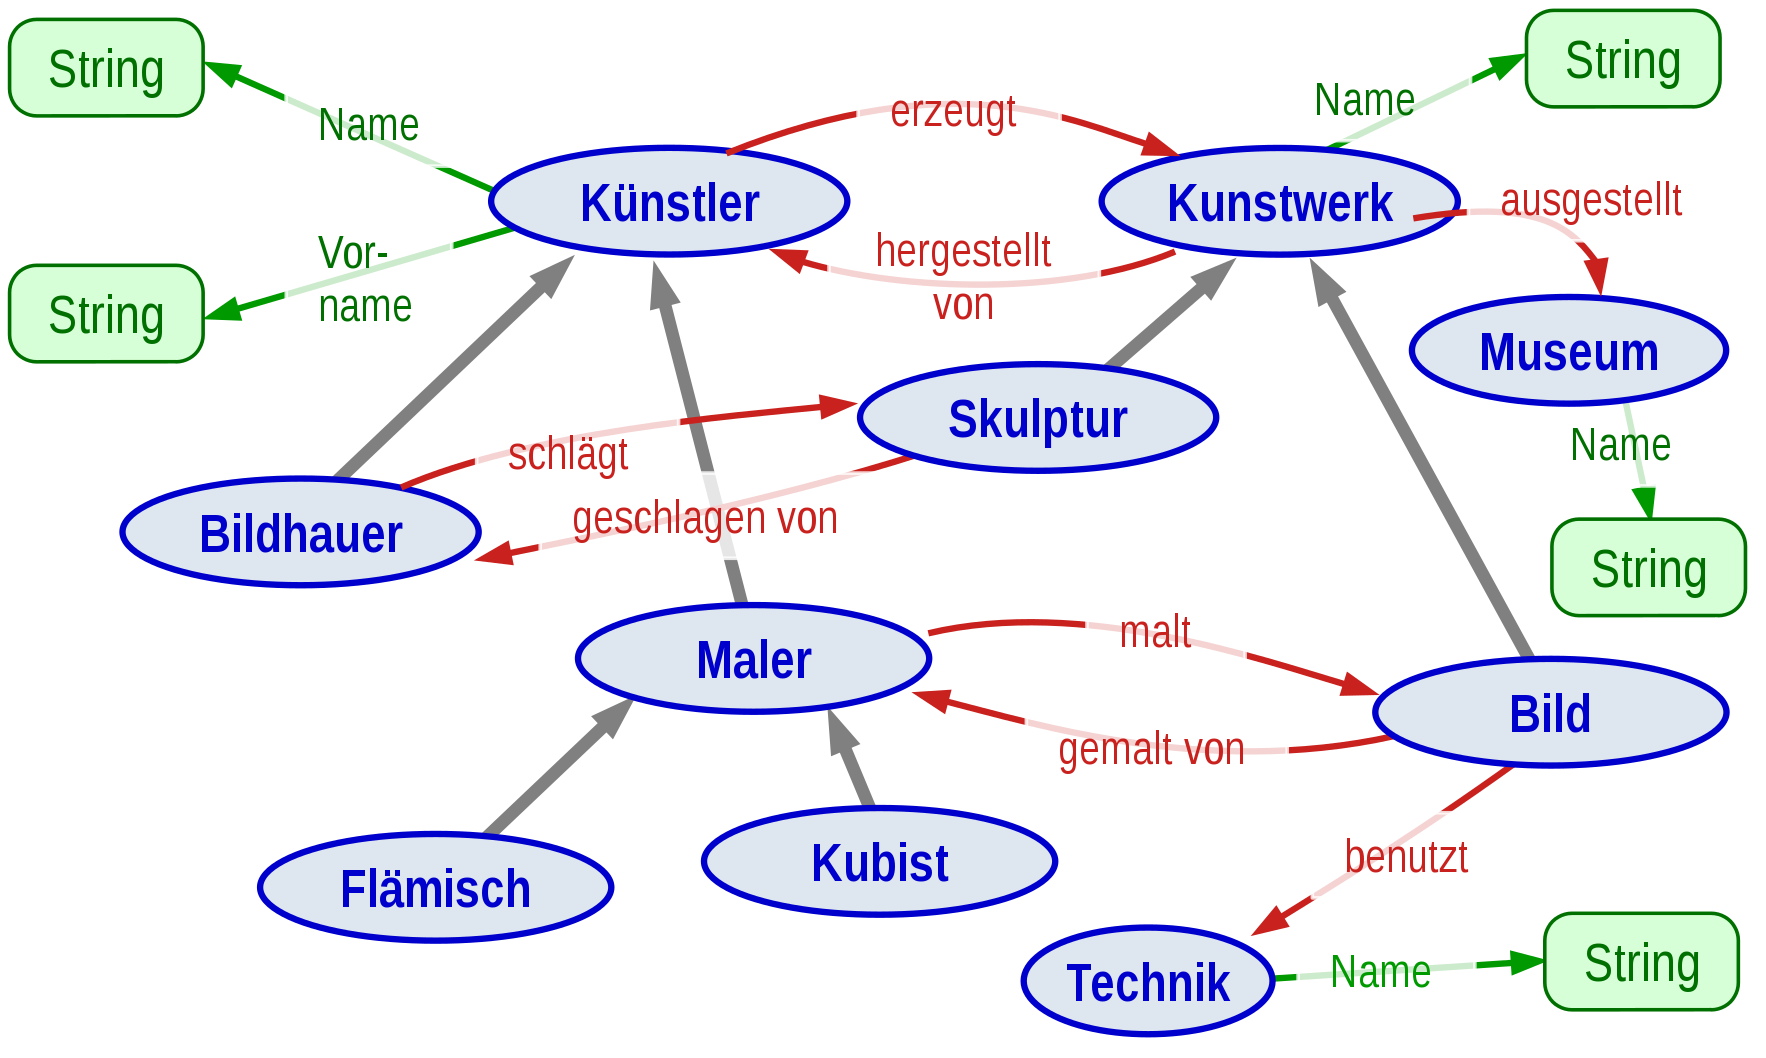
\includegraphics[height=0.7\textheight]{graphics/onto_typ}\\
  \Viertelzeile
  \grau{\tiny Quelle \url{https://de.wikipedia.org/wiki/Ontologie\_(Informatik)\#/media/Datei:Ontschichten.svg}}
\end{frame}

\begin{frame}
  {Ontologisch klassifizierte Objekte}
  \onslide<+->
  \centering
  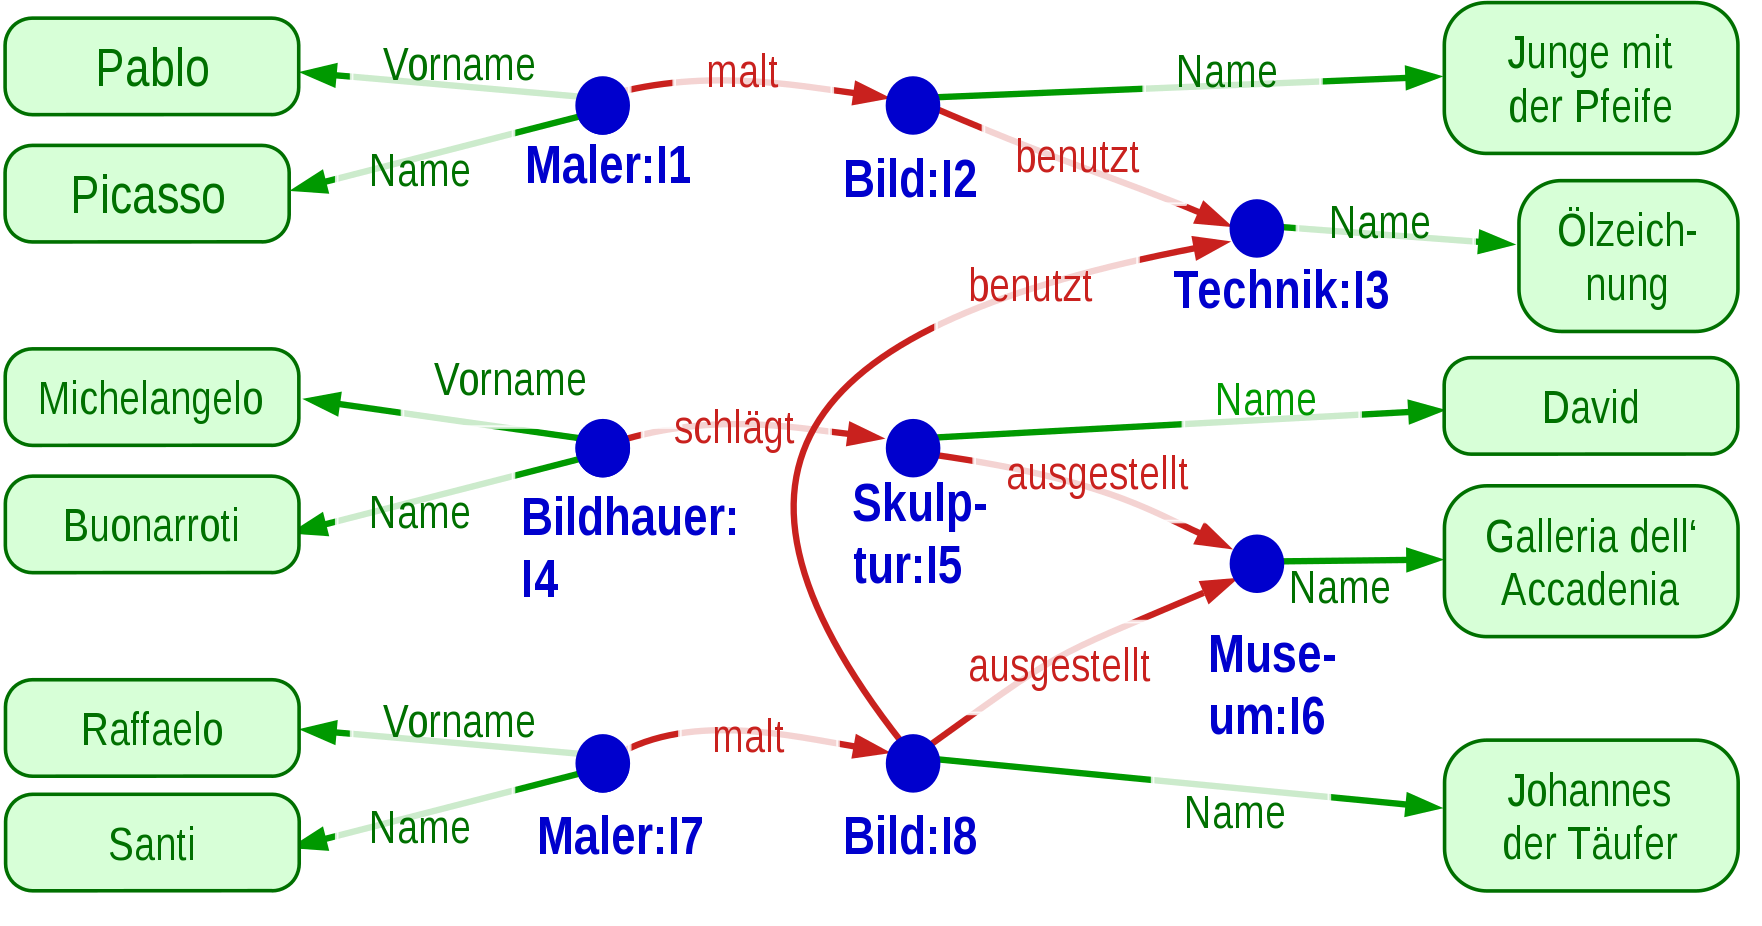
\includegraphics[height=0.7\textheight]{graphics/onto_tok}\\
  \Viertelzeile
  \grau{\tiny Quelle \url{https://de.wikipedia.org/wiki/Ontologie\_(Informatik)\#/media/Datei:Ontschichten.svg}}
\end{frame}

\section{Morphologie}

\begin{frame}
  {Wortklassen und Veränderlichkeit}
  \onslide<+->
  Was für Wortklassen gibt es, und was unterscheidet sie \alert{grammatisch}?\\
  \onslide<+->
  \Zeile
  \begin{itemize}[<+->]
    \item Veränderlichkeit (Flexion und Wortbildung)
    \item mögliche Arten der Veränderlichkeit
    \item syntaktisches Kombinierbarkeit
    \item \ldots
  \end{itemize}
\end{frame}

\begin{frame}
  {Form und Funktion | Flexion}
  \pause
  \begin{exe}
    \ex
    \begin{xlist}
      \ex \alert{Den Präsidenten} begrüßte \alert{der Dekan} äußerst respektlos.
      \pause
      \ex \alert{Der Dekan} begrüßte \alert{den Präsidenten} äußerst respektlos.
    \end{xlist}
    \pause
    \ex
    \begin{xlist}
      \ex \alert{Die Präsidentin} begrüßte \alert{die Dekanin} äußerst respektlos.
      \pause
      \ex \alert{Die Dekanin} begrüßte \alert{die Präsidentin} äußerst respektlos.
    \end{xlist}
  \end{exe}
  \pause
  \Zeile
  Formveränderungen lexikalischer Wörter \alert{schränken ihre möglichen grammatischen Funktionen und Relationen im Satz ein}\dots\\
  \pause
  \Halbzeile
  \dots und sie haben semantische und systemexterne Folgen.
\end{frame}

\begin{frame}
  {Unterklassen | Beispiel Substantive}
  \onslide<+->
  Wie gliedert sich der substantivische Wortschatz weiter?
  \onslide<+->
  \Zeile
  \begin{itemize}[<+->]
    \item \alert{Genus} | Maskulinum, Neutrum, Femininum
    \item Maskulinum | \alert{stark}, \alert{schwach}, \alert{gemischt} (oder so ähnlich)
    \item Femininum | Plural mit \textit{-e}, \textit{-en} oder endunglos (oder so ähnlich) 
  \end{itemize}
\end{frame}

\begin{frame}
  {Form und Funktion | Wortbildung}
  \pause
  \begin{exe}
    \ex grün\alert{lich}, röt\alert{lich}, gelb\alert{lich}
    \pause
    \ex Neu\alert{igkeit}, Blöd\alert{heit}, Tauch\alert{er}, Heb\alert{ung}
    \pause
    \ex Fenster\alert{rahmen}, Tücher\alert{spender}, Glas\alert{korken}, Unter\alert{schrank}
  \end{exe}
  \pause
  \Zeile
  Formveränderungen von einem zu einem anderen lexikalischen Wort führen zu Bedeutungs- und kategorialen Veränderungen.
\end{frame}


\section{Struktur im Lexikon | Form}

\begin{frame}
  {Wortklassen | Morphosyntaktische Vorstrukturierung}
  \centering
  \resizebox{0.35\textwidth}{!}{
  \begin{minipage}{\textwidth}
  \centering
  \begin{forest}
    /tikz/every node/.append style={font=\footnotesize},
    for tree={l sep=2em, s sep=2.5em},
    [\textit{Wort}, intrme
      [{Hat\\Numerus?}, decide
        [\textit{flektierbar}, intrme, yes
          [{Ist finit\\flektierbar?}, decide
            [\textbf{Verb}, finall, yes]
            [\textit{Nomen}, intrme, no
              [{Hat festes\\Genus?}, decide
                [\textbf{Substantiv}, finall, yes]
                [{\textit{anderes}\\\textit{Nomen}}, intrme, no
                  [{Hat Stärke-\\flexion?}, decide
                    [\textbf{Adjektiv}, finall, yes]
                    [{\textit{Artikel\slash}\\\textit{Pronomen}}, intrme, no]
                  ]
                ]
              ]
            ]
          ]
        ]
        [\textit{nicht flektierbar}, intrme, no
        [{Hat Valenz-\slash\\Kasusrektion?}, decide
            [\textbf{Präposition}, finall, yes]
            [\textit{andere}, intrme, no
              [{Leitet Neben-\\Sätze ein?}, decide
                [\textbf{Komplementierer}, finall, yes]
                [{\textit{Partikel\slash}\\\textit{Adverb}}, intrme, no
                  [{Kann das Vor-\\feld besetzen?}, decide
                    [{\textit{Adverb\slash}\\\textit{Adkopula}}, intrme, yes
                      [{Wird typisch mit\\Kopula verwendet?}, decide
                        [\textbf{Adkopula}, finall, yes]
                        [\textbf{Adverb}, finall, no]
                      ]
                    ]
                    [\textit{Partikel}, intrme, no
                      [{Kann Sätze\\ersetzen?}, decide
                        [\textbf{Satzäquivalent}, finall, yes]
                        [\textit{andere}, intrme, no
                          [{Kann Konsti-\\tuenten verbinden?}, decide
                            [\textbf{Konjunktion}, finall, yes]
                            [\textit{Rest}, intrme, no]
                          ]
                        ]
                      ]
                    ]
                  ]
                ]
              ]
            ]
          ]
        ]
      ]
    ]
  \end{forest}
  \end{minipage}
  }
\end{frame}



\begin{frame}
  {Flexionsklassen der Substantive | Traditionell}
  \onslide<+->
  \centering
  \resizebox{0.8\textwidth}{!}{
        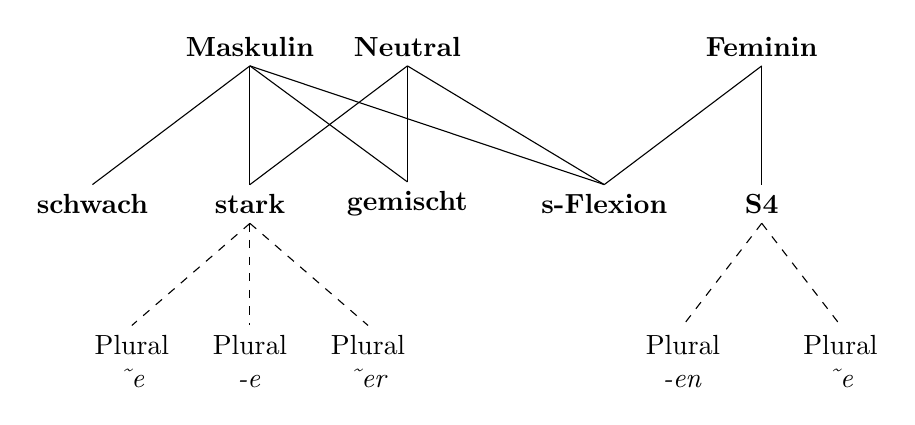
\begin{tikzpicture}[every text node part/.style={align=center}]
      \node (MaskN)    at (2,4)   {\textbf{Maskulin}};
      \node (NeutN)    at (4,4)   {\textbf{Neutral}};
      \node (FemN)     at (8.5,4) {\textbf{Feminin}};

      \node (schwachN) at (0,2)   {\textbf{schwach}};
      \node (starkN)   at (2,2)   {\textbf{stark}};
      \node (gemistN)  at (4,2)   {\textbf{gemischt}};
      \node (sFlexN)   at (6.5,2) {\textbf{s-Flexion}};
      \node (s4N)      at (8.5,2) {\textbf{S4}};

      \node (EPlu)     at (0.5,0) {Plural\\\textit{\char`~e}};
      \node (ePlu)     at (2,0)   {Plural\\\textit{-e}};
      \node (erPlu)    at (3.5,0) {Plural\\\textit{\char`~er}};

      \node (enPlu)    at (7.5,0) {Plural\\\textit{-en}};
      \node (EnPlu)    at (9.5,0) {Plural\\\textit{\char`~e}};

      \draw (MaskN.south)  -- (schwachN.north);
      \draw (MaskN.south)  -- (starkN.north);
      \draw (MaskN.south)  -- (gemistN.north);
      \draw (MaskN.south)  -- (sFlexN.north);

      \draw (NeutN.south)  -- (starkN.north);
      \draw (NeutN.south)  -- (gemistN.north);
      \draw (NeutN.south)  -- (sFlexN.north);

      \draw (FemN.south)   -- (s4N.north);
      \draw (FemN.south)   -- (sFlexN.north);

      \draw [dashed] (starkN.south) -- (EPlu.north);
      \draw [dashed] (starkN.south) -- (ePlu.north);
      \draw [dashed] (starkN.south) -- (erPlu.north);

      \draw [dashed] (s4N.south)    -- (enPlu.north);
      \draw [dashed] (s4N.south)    -- (EnPlu.north);
    \end{tikzpicture}
  \begin{minipage}{\textwidth}
  \centering 
  \end{minipage}
  }
\end{frame}

\begin{frame}
  {Flexionsklassen der Substantive | Revidiert}
  \onslide<+->
  \centering
  \resizebox{0.8\textwidth}{!}{
  \begin{minipage}{\textwidth}
  \centering 
    \begin{forest}
    [Substantive, calign=last, l sep+=2em
      [\textit{en}-Maskulina]
      [normale Flexion{,}\\differenziert\\nur nach\\Pluralbildung, l sep+=2em
        [\textit{\char`~er}\\nur Maskulina\\und Neutra\\(Kleinstklasse)]
        [\textit{\char`~e}\slash\textit{-e}\\Protoyp\\der \textbf{Maskulina}\\und \textbf{Neutra}]
        [\textit{-en}\\Prototyp\\der \textbf{Feminina}]
        [\textit{-s}\\lexikalisch oder\\phonotaktisch\\motiviert]
      ]
    ]
  \end{forest}
  \end{minipage}
  }
\end{frame}



